\section{\name: a Secure Embedded OS}
\label{sec:os}

\name is a new embedded operating system
specifically designed for platforms running multiple, potentially untrusted
applications concurrently and third-party, contributed device drivers that are
assumed to be buggy. \name uses three protection mechanisms to protect three
different components in the operating system.
First, the kernel is written in Rust~\cite{rust}, a new systems language that provides
compile-time memory safety and ownership, and uses the language to protect the
core of the kernel (e.g. the scheduler and hardware abstraction layer) from
contributed device drivers.
Second, \name uses new Memory Protection Units (MPUs) to isolate third-party
applications from each other and the kernel.
Finally, where available, \name uses multiple microcontrollers to protect
applications with timing concerns against starvation or leaking side-channel
information.
The remainder of this section gives an overview of the \name architecture,
and aims to provide some intuition for importance and usage of an MPU.

\subsection{Architecture}
\label{sec:os-arch}

% Definitions:
%  Tock core -- the kernel code shipped and provided with base Tock
%  Tock kernel -- the final compiled kernel, including core and drivers

Unlike traditional, monolithic embedded operating systems, \name generates a
standalone, portable kernel that is composed of platform-specific drivers at
compile-time and enables dynamic loading of third-party applications at
runtime.

The \name core has complete system access, including arbitrary memory
access and interrupt control. Device drivers are compiled into the kernel and
run with the same \emph{hardware} privileges but inside a
\emph{language-level} sandbox. This sandbox statically enforces that device
drivers only use core-provided hardware interfaces, limits dynamic memory
allocation to load time, and prevents uncoordinated access of underlying
hardware resources.

Applications are separated from the kernel by a syscall ABI and need not be
written in Rust. Applications have an execution stack, an application memory
heap, and a kernel memory heap. Kernel (and driver) dynamic allocations take
place in the application memory space, thus charging applications for buffers
the kernel creates on their behalf and ensuring that an out-of-memory
condition terminates the application and does not cause a kernel error. The
application-level kernel memory heap is protected from application access by the
MPU.
%
The ABI provides access to system hardware resources. For embedded applications,
however, direct access to a hardware peripheral is often required.
Applications can request direct ownership, in which case the kernel uses the
MPU to grant the application access to the memory mapped I/O region of
specific peripherals.

%% Brad: not sure what this paragraph contributes to the paper, particularly
%% in this section. I think the contents of this should be discussed in the sections above, if
%% at all.
% Scheduling in \name is an open question, particularly if it aims to capitalize
% on multi-MCU systems. Some assignments are clearer, a communication task
% should likely run on the same core as the radio controller. Applications
% that require hard real-time could run on a dedicated core with a real-time
% scheduler, but what if another core is not available? Technology such as
% TrustZone~\cite{trustzone}, a secure processing mode on the same physical
% core, provides protection for sensitive data, but not from side-channel
% attacks such as timing.


% TrustZone is interesting, but currently only available on Cortex-A's, not
% clear if there's any intention of bringing to M's. Maybe this though belongs
% more in the HW section earlier?


% \subsection{The Cortex-M MPU}
%
% The Cortex-M MPU allows the kernel to defined eight memory regions. Each memory
% region may be sized between 32 bytes and 4GB, in 32 byte increments and has
% protection bits for read, write and execute. Regions may overlap, in which case
% the memory region with the highest number ``wins''. In addition, regions of at
% least 256 bytes can be divided into eight equal sized subregions, which can
% either be turned on---in which case they inheret the parent region's protection
% bits---or turned off---in which case the parent's protection bits do not apply.
% As a result, the operating system can control access to up to 64 concurrently
% active regions. Finally, memory regions and protection bits can be changed
% during exection, for example while context switching between applications.


\subsection{\name Memory Design in Detail}

\begin{figure}
 \centering
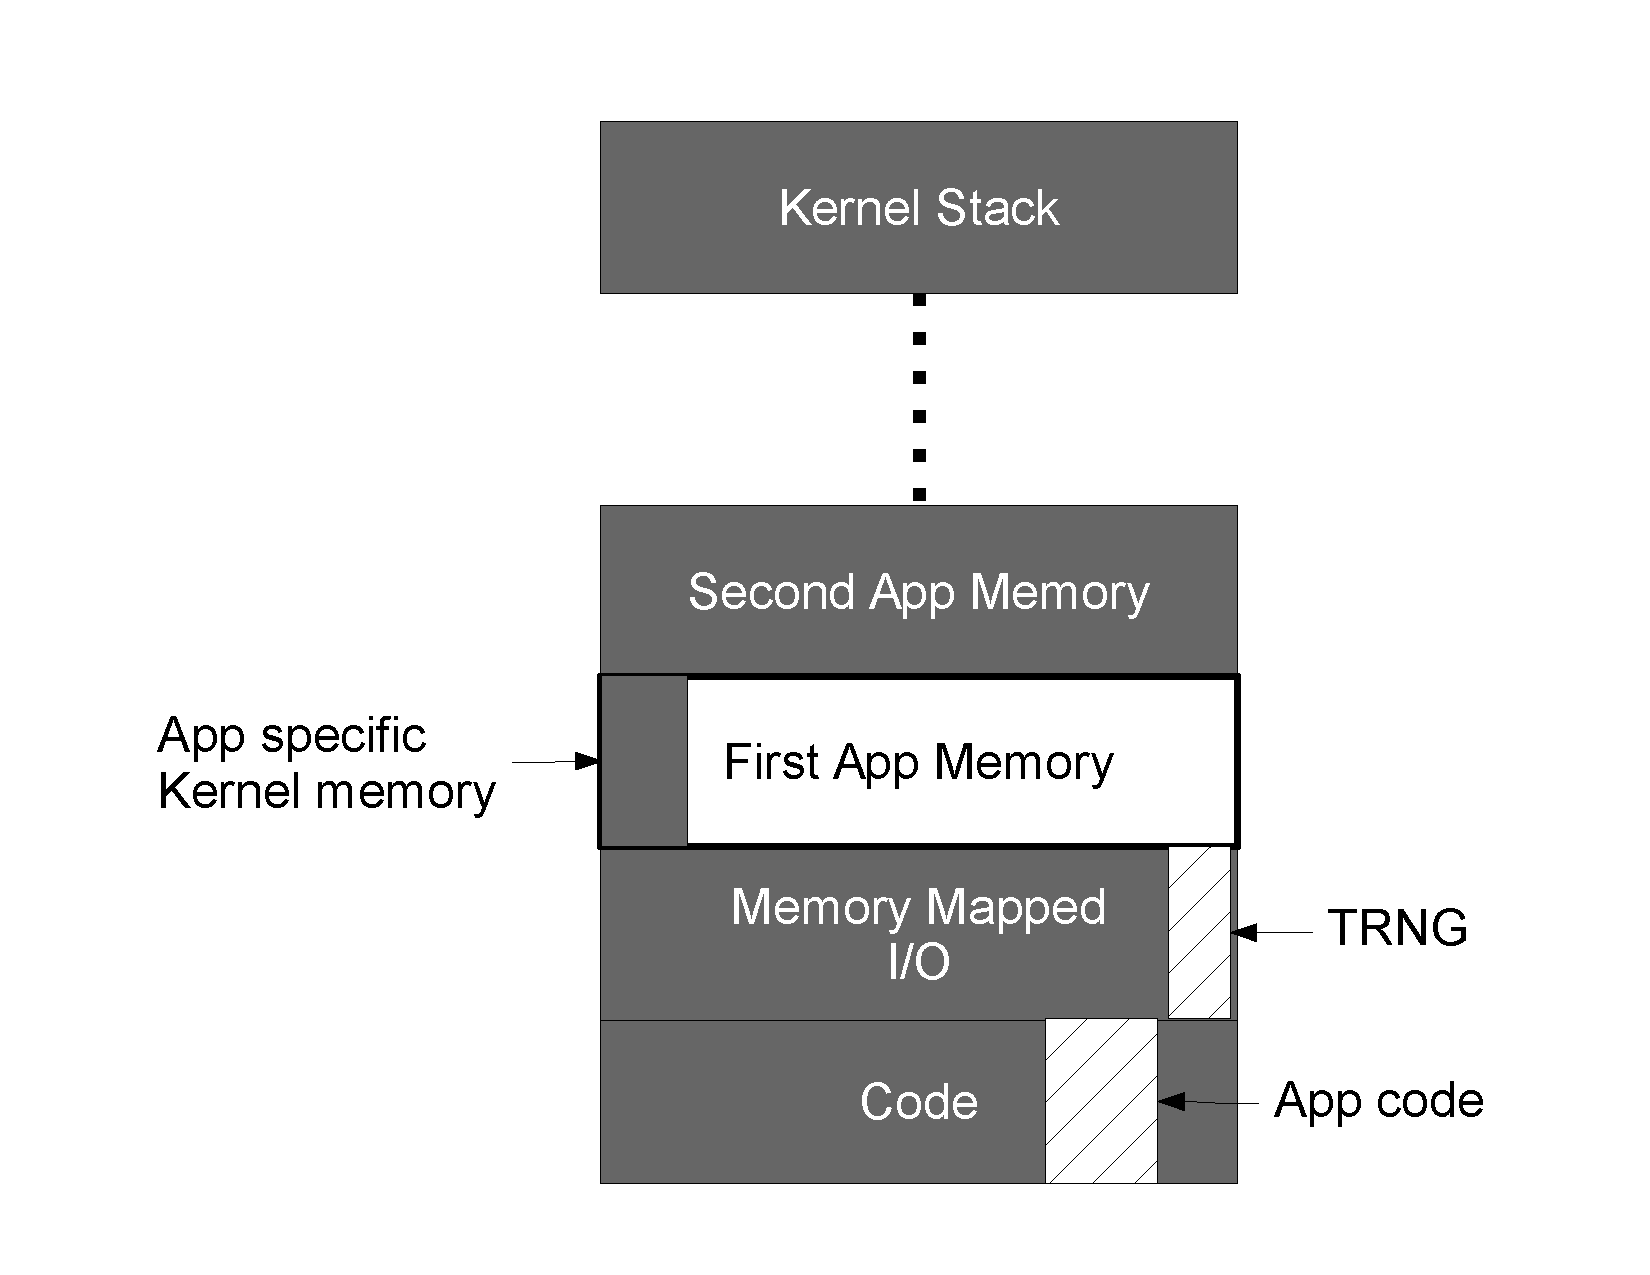
\includegraphics[width=1\columnwidth]{img/memory-layout}
\caption{Memory layout and access permissions while executing an application.
\name lays out memory into four types of regions: code, memory mapped I/O,
application memory and the kernel stack. Greyed regions are marked unreadable
and unwritable, while hatched regions are read-only. The application memory
contains a subregion used by the kernel for application-specific kernel data
structures and is thus inaccessible to the application. Conversely, some
hardware registers are exposed directly to applications by marking them
read-only.}
 \label{fig:memory-layout}
\end{figure}

Without virtual memory but the requirement of providing memory isolation
between applications and the kernel, \name has a carefully designed memory
architecture.  \Cref{fig:memory-layout} shows the four types of memory
regions in \name and the access rules during application execution.

{\bf Code.}
The code region contains kernel and application code.  While an application is
executing code, it only has read and instruction fetch access to its own code
segment.  An application cannot write to its own code section
because typically
% since, in most cases,
the code is backed by internal flash, which has limited write cycles.

% n.b. Why endnotes? I looked around the HotOS CFP, and couldn't find anything
% that requires them over footnotes. They're much more annoying to read IMHO.
{\bf Memory-Mapped I/O.}
Hardware registers are typically located in a single, continuous region of the
memory space.~\endnote{The location of hardware memory registers and flash is
  determined by the chip manufacturer, however, chips chips typically place
  flash at the bottom of memory, followed by RAM, and peripheral memory
registers towards the top of memory.}
\name may provide read-only or read-write access over small ranges of memory
registers to applications, bypassing the kernel for direct hardware access.
For example, our development platform uses the Atmel SAM4L Cortex-M4~\cite{sam4l} which
provides a true random number generator (TRNG) peripheral.
\name exposes random
numbers directly to applications by allowing read-only access to a 32~byte
range covering the 20~byte long TRNG registers (the tailing 12 bytes are innocuous).
% The registers for reading
% a new random value are contained in an 20~byte range.  \name exposes random
% numbers directly to applications by allowing read-only access to a 32~byte
% range covering these registers (the tailing 12 bytes are innocuous).

{\bf Kernel Stack and Static Data.}
This section includes all kernel and device driver memory, including local
variables. The MPU restricts any application-level access to this memory section.
% buffers and any local
% variables such that applications may not access the kernel stack in any way.
% The kernel does not allocate memory dynamically except on the stack and inside
% application memory regions.
%As a result, the kernel stack is the only region dedicated to kernel memory.

{\bf Application Memory.}
Currently, \name allocates a continuous, fixed size region for each
application.
%(our development platform has 64KB of RAM and we currently use 2KB
%memory regions for applications, but this will likely vary based on the
%requirements of each target platform).
Application memory and the kernel stack grow towards each other to balance
application count with kernel stack size. If the kernel stack
grows too large, \name terminates the application with the
largest memory region. We intend to explore an alternate strategy of
allocating application memory from a shared heap using the
high granularity of the MPU.
This would trade-off
% We have not yet explored the tradeoffs between
% these two strategies, but at a high level fixed sized application memory
% regions make it
a simpler processes for reclaiming stack space
for better support of heterogeneously sized applications.


An application's memory region is not entirely its own. Most of its memory is
used for its stack, static variables, and heap. However,
the kernel may also ``borrow'' memory from the top of an application's memory
region for application-specific kernel data structures. This region, which may
change in size,
%is \emph{inside} the application's memory space, but
is marked
as read and write protected when the application is running. Therefore, the
kernel and device drivers can allocate memory dynamically in response to an
application without
potentially causing an out-of-memory kernel error and while still
% sacrificing the reliability of never dynamically
% allocating in the kernel itself and while
maintaining the integrity and
confidentiality of shared kernel data structures. As an example, when an
application registers a callback for a timer, the timer device driver
allocates a new link node for the callback in the application's memory.
% adds the
% request to its list of pending timers by allocating the new list node in the
% application's memory.
Since the link includes forward and backward list
pointers, it is imperative that, despite being in the application's memory,
this link's integrity be maintained. Moreover, the values of the links might
leak information about other applications.

